\documentclass{ximera}
\usepackage{sagetex}
%% handout
%% space
%% newpage
%% numbers
%% nooutcomes

%% You can put user macros here
%% However, you cannot make new environments

\graphicspath{{./}{module1Activity/}{module2Activity/}{module3Activity/}}

\usepackage{sagetex}
\usepackage{tikz}
\usepackage{hyperref}
\usepackage{tkz-euclide}
\usetkzobj{all}
\pgfplotsset{compat=1.7} % prevents compile error.

\tikzstyle geometryDiagrams=[ultra thick,color=blue!50!black]
 %% we can turn off input when making a master document

\outcome{}
\author{Darryl Chamberlain Jr.}
 
\title{Objective 1 - End and Zero Behavior}

\begin{document}
\begin{abstract}
Identify the end behavior and zero behavior of a polynomial function.
\end{abstract}
\maketitle

\href{https://cnx.org/contents/mwjClAV_@8.1:ZE9qk3Qp@12/Graphs-of-Polynomial-Functions}{Link to section in online textbook.}

%%%%%%%%%%%%%%%%%%%%%
%%%  Objective 1  %%%
%%%%%%%%%%%%%%%%%%%%%

First, watch \underline{\href{https://mediasite.video.ufl.edu/Mediasite/Play/8814f4cd9bc24a2ea1f4cee8e42f09b21d}{this video}} to learn how to identify the end behavior and zero behavior of polynomial functions. Now practice describing the end behavior and zero behavior of polynomials below. 

\begin{sagesilent}
x = var("x")
def maybeMakeNegative(natural):
    integer = (-1)**ZZ.random_element(2)
    return integer 

def listZeros(factor1, factor2):
    z0 = factor1
    z1 = -factor1
    z2 = factor2
    z3 = -factor2
    return [z0, z1, z2, z3]

def generateCoefficientsAndZeros():
    leadingCoefficient = maybeMakeNegative(ZZ.random_element(2, 10))
    factor1 = ZZ.random_element(2, 10)
    factor2 = ZZ.random_element(2, 10)
    while factor1 == factor2:
        factor1 = ZZ.random_element(2, 10)
        factor2 = ZZ.random_element(2, 10)
    chooseZero = ZZ.random_element(2)
    if chooseZero == 0:
        zeroOnDisplay = -factor1
        e0 = ZZ.random_element(1, 4)
        e1 = e0 + 2 * ZZ.random_element(1, 4) - 1
        e2 = ZZ.random_element(1, 4)
        e3 = e2 + ZZ.random_element(0, 3)
    else: 
        zeroOnDisplay = -factor2
        e0 = ZZ.random_element(1, 4)
        e1 = e0 + ZZ.random_element(0, 3)
        e2 = ZZ.random_element(1, 4)
        e3 = e2 + 2 * ZZ.random_element(1, 4) - 1
    zeros = listZeros(factor1, factor2)
    exponents = e0, e1, e2, e3
    return [leadingCoefficient, zeros, exponents, zeroOnDisplay]

def displayPolynomial(leadingCoefficient, zeros, exponents):
    z0, z1, z2, z3 = zeros
    e0, e1, e2, e3 = exponents 
    polynomial = leadingCoefficient * (x - z0)**e0 * (x - z1)**e1 * (x - z2)**e2 * (x - z3)**e3
    return polynomial 

def endBehaviorAnswer(leadingCoefficient, exponents):
    e0, e1, e2, e3 = exponents 
    evenOrOdd = (e0 + e1 + e2 + e3) % 2 
    if leadingCoefficient < 0 and evenOrOdd == 1:
        answer = "A"
    elif leadingCoefficient < 0 and evenOrOdd == 0:
        answer = "B"
    elif leadingCoefficient > 0 and evenOrOdd == 1:
        answer = "C"
    elif leadingCoefficient > 0 and evenOrOdd == 0:
        answer = "D"
    else: 
        answer = "Broken"
    return answer 

def zeroBehaviorAnswer(polynomial, zeroOnDisplay, exponentOnDisplay): 
    nearZero = zeroOnDisplay - 0.5
    yValue = polynomial(x = nearZero)
    evenOrOdd = exponentOnDisplay % 2
    if yValue > 0 and evenOrOdd == 0:
        answer = "EvenPositive"
    elif yValue > 0 and evenOrOdd == 1:
        answer = "OddNegative"
    elif yValue < 0 and evenOrOdd == 0:
        answer = "EvenNegative"
    else:
        answer = "OddPositive"
    return answer

def findDisplayExponent(zeroOnDisplay, zeros, exponents):
    z0, z1, z2, z3 = zeros
    e0, e1, e2, e3 = exponents
    if zeroOnDisplay == z0:
        return e0
    elif zeroOnDisplay == z1: 
        return e1 
    elif zeroOnDisplay == z2:
        return e2
    else:
        return e3
    
### Question 2 - Answer B ###
leadingCoefficient2, zeros2, exponents2, zeroOnDisplay2 = generateCoefficientsAndZeros()
polynomial2 = displayPolynomial(leadingCoefficient2, zeros2, exponents2)
answer2 = endBehaviorAnswer(leadingCoefficient2, exponents2)
while answer2 == "A" or answer2 == "C" or answer2 == "D":
    leadingCoefficient2, zeros2, exponents2, zeroOnDisplay2 = generateCoefficientsAndZeros()
    polynomial2 = displayPolynomial(leadingCoefficient2, zeros2, exponents2)
    answer2 = endBehaviorAnswer(leadingCoefficient2, exponents2)

### Question 3 - Answer D ###
leadingCoefficient3, zeros3, exponents3, zeroOnDisplay3 = generateCoefficientsAndZeros()
polynomial3 = displayPolynomial(leadingCoefficient3, zeros3, exponents3)
answer3 = endBehaviorAnswer(leadingCoefficient3, exponents3)
while answer3 == "A" or answer3 == "B" or answer3 == "C":
    leadingCoefficient3, zeros3, exponents3, zeroOnDisplay3 = generateCoefficientsAndZeros()
    polynomial3 = displayPolynomial(leadingCoefficient3, zeros3, exponents3)
    answer3 = endBehaviorAnswer(leadingCoefficient3, exponents3)

### Question 4 - Answer A ###
leadingCoefficient4, zeros4, exponents4, zeroOnDisplay4 = generateCoefficientsAndZeros()
polynomial4 = displayPolynomial(leadingCoefficient4, zeros4, exponents4)
answer4 = endBehaviorAnswer(leadingCoefficient4, exponents4)
while answer4 == "B" or answer4 == "C" or answer4 == "D":
    leadingCoefficient4, zeros4, exponents4, zeroOnDisplay4 = generateCoefficientsAndZeros()
    polynomial4 = displayPolynomial(leadingCoefficient4, zeros4, exponents4)
    answer4 = endBehaviorAnswer(leadingCoefficient4, exponents4)

### Question 5 - Answer C ###
leadingCoefficient5, zeros5, exponents5, zeroOnDisplay5 = generateCoefficientsAndZeros()
polynomial5 = displayPolynomial(leadingCoefficient5, zeros5, exponents5)
answer5 = endBehaviorAnswer(leadingCoefficient5, exponents5)
while answer5 == "A" or answer5 == "B" or answer5 == "D":
    leadingCoefficient5, zeros5, exponents5, zeroOnDisplay5 = generateCoefficientsAndZeros()
    polynomial5 = displayPolynomial(leadingCoefficient5, zeros5, exponents5)
    answer5 = endBehaviorAnswer(leadingCoefficient5, exponents5)

##### Question 6 - Odd Negative #####
leadingCoefficient6, zeros6, exponents6, zeroOnDisplay6 = generateCoefficientsAndZeros()
polynomial6 = displayPolynomial(leadingCoefficient6, zeros6, exponents6)
exponentOnDisplay6 = findDisplayExponent(zeroOnDisplay6, zeros6, exponents6)
answer6 = zeroBehaviorAnswer(polynomial6, zeroOnDisplay6, exponentOnDisplay6)

while answer6 == "EvenPositive" or answer6 == "EvenNegative" or answer6 == "OddPositive":
    leadingCoefficient6, zeros6, exponents6, zeroOnDisplay6 = generateCoefficientsAndZeros()
    polynomial6 = displayPolynomial(leadingCoefficient6, zeros6, exponents6)
    exponentOnDisplay6 = findDisplayExponent(zeroOnDisplay6, zeros6, exponents6)
    answer6 =  zeroBehaviorAnswer(polynomial6, zeroOnDisplay6, exponentOnDisplay6)

##### Question 7 - Even Negative #####
leadingCoefficient7, zeros7, exponents7, zeroOnDisplay7 = generateCoefficientsAndZeros()
polynomial7 = displayPolynomial(leadingCoefficient7, zeros7, exponents7)
exponentOnDisplay7 = findDisplayExponent(zeroOnDisplay7, zeros7, exponents7)
answer7 = zeroBehaviorAnswer(polynomial7, zeroOnDisplay7, exponentOnDisplay7)
while answer7 == "EvenPositive" or answer7 == "OddNegative" or answer7 == "OddPositive":
    leadingCoefficient7, zeros7, exponents7, zeroOnDisplay7 = generateCoefficientsAndZeros()
    polynomial7 = displayPolynomial(leadingCoefficient7, zeros7, exponents7)
    exponentOnDisplay7 = findDisplayExponent(zeroOnDisplay7, zeros7, exponents7)
    answer7 =  zeroBehaviorAnswer(polynomial7, zeroOnDisplay7, exponentOnDisplay7)

##### Question 8 - Even Positive #####
leadingCoefficient8, zeros8, exponents8, zeroOnDisplay8 = generateCoefficientsAndZeros()
polynomial8 = displayPolynomial(leadingCoefficient8, zeros8, exponents8)
exponentOnDisplay8 = findDisplayExponent(zeroOnDisplay8, zeros8, exponents8)
answer8 = zeroBehaviorAnswer(polynomial8, zeroOnDisplay8, exponentOnDisplay8)
while answer8 == "EvenNegative" or answer8 == "OddNegative" or answer8 == "OddPositive":
    leadingCoefficient8, zeros8, exponents8, zeroOnDisplay8 = generateCoefficientsAndZeros()
    polynomial8 = displayPolynomial(leadingCoefficient8, zeros8, exponents8)
    exponentOnDisplay8 = findDisplayExponent(zeroOnDisplay8, zeros8, exponents8)
    answer8 =  zeroBehaviorAnswer(polynomial8, zeroOnDisplay8, exponentOnDisplay8)

##### Question 9 - Odd Positive #####
leadingCoefficient9, zeros9, exponents9, zeroOnDisplay9 = generateCoefficientsAndZeros()
polynomial9 = displayPolynomial(leadingCoefficient9, zeros9, exponents9)
exponentOnDisplay9 = findDisplayExponent(zeroOnDisplay9, zeros9, exponents9)
answer9 = zeroBehaviorAnswer(polynomial9, zeroOnDisplay9, exponentOnDisplay9)
while answer9 == "EvenPositive" or answer9 == "OddNegative" or answer9 == "EvenNegative":
    leadingCoefficient9, zeros9, exponents9, zeroOnDisplay9 = generateCoefficientsAndZeros()
    polynomial9 = displayPolynomial(leadingCoefficient9, zeros9, exponents9)
    exponentOnDisplay9 = findDisplayExponent(zeroOnDisplay9, zeros9, exponents9)
    answer9 =  zeroBehaviorAnswer(polynomial9, zeroOnDisplay9, exponentOnDisplay9)
\end{sagesilent}

% Q2
\begin{question}
Choose the \textbf{end behavior} of the polynomial below.

$$ f(x) = \sage{polynomial2} $$

\begin{center}
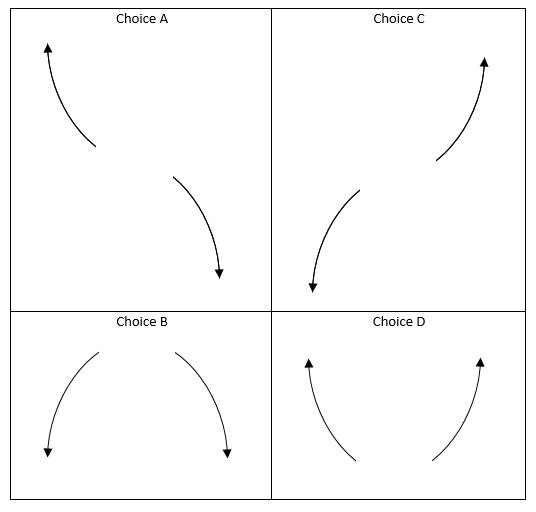
\includegraphics[scale=0.5]{endBehaviorOptions.png}
\end{center}

\begin{multipleChoice}
    \choice A Choice A \\
    \choice[correct] B Choice B \\
    \choice C Choice C \\
    \choice D Choice D
\end{multipleChoice}

\end{question}

% Q3
\begin{question}
Choose the \textbf{end behavior} of the polynomial below.

$$ f(x) = \sage{polynomial3} $$

\begin{center}
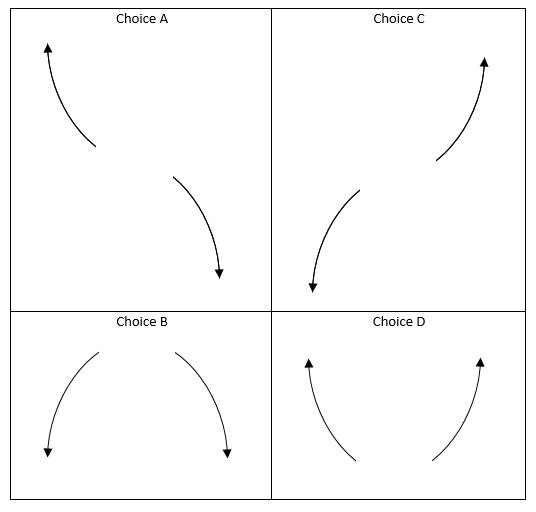
\includegraphics[scale=0.5]{endBehaviorOptions.png}
\end{center}

\begin{multipleChoice}
    \choice A Choice A \\
    \choice B Choice B \\
    \choice C Choice C \\
    \choice[correct] D Choice D
\end{multipleChoice}

\end{question}

% Q4
\begin{question}
Choose the \textbf{end behavior} of the polynomial below.

$$ f(x) = \sage{polynomial4} $$

\begin{center}
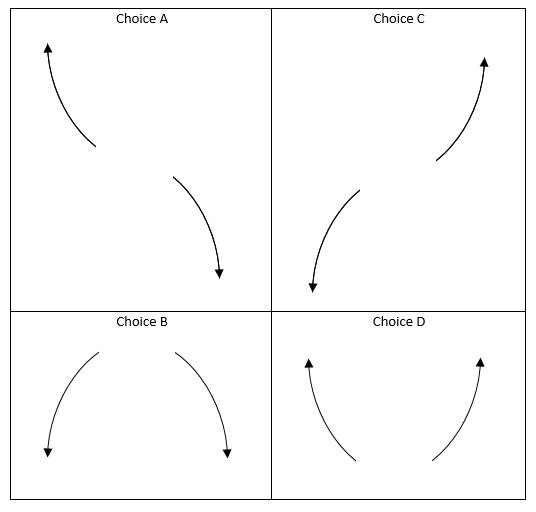
\includegraphics[scale=0.5]{endBehaviorOptions.png}
\end{center}

\begin{multipleChoice}
    \choice[correct] A Choice A \\
    \choice B Choice B \\
    \choice C Choice C \\
    \choice D Choice D
\end{multipleChoice}

\end{question}

% Q5
\begin{question}
Choose the \textbf{end behavior} of the polynomial below.

$$ f(x) = \sage{polynomial5} $$

\begin{center}
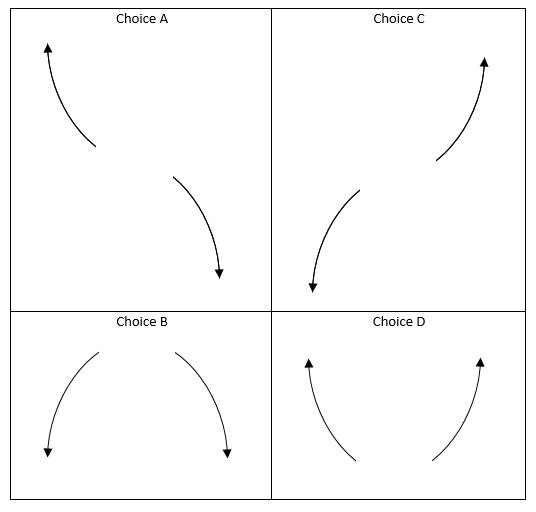
\includegraphics[scale=0.5]{endBehaviorOptions.png}
\end{center}

\begin{multipleChoice}
    \choice A Choice A \\
    \choice B Choice B \\
    \choice[correct] C Choice C \\
    \choice D Choice D
\end{multipleChoice}

\end{question}

% Q6
\begin{question}
Choose the option that describes the behavior at $x = \sage{zeroOnDisplay6}$ of the polynomial below.

$$ f(x) =  \sage{polynomial6} $$

\begin{center}
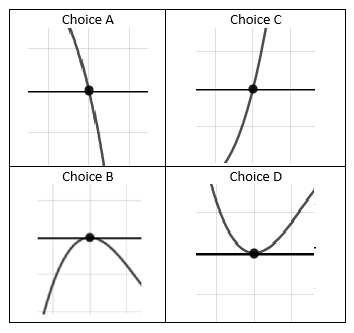
\includegraphics[scale=0.75]{zeroBehaviorOptions.png}
\end{center}

\begin{multipleChoice}
    \choice[correct] A Choice A \\
    \choice B Choice B \\
    \choice C Choice C \\
    \choice D Choice D
\end{multipleChoice}

\begin{hint}
To know \textbf{exactly} what the zero behavior is, we should sketch the entire function. Clever students may figure out an arithmetic way to check zero behavior, but it is easier to sketch the function using end behavior and multiplicity of the zeros. \href{https://www.youtube.com/watch?v=-3vPQ_mx1vY}{Here is an example video for this particular type of problem.}
\end{hint}

\end{question}

% Q7
\begin{question}
Choose the option that describes the behavior at $x = \sage{zeroOnDisplay7}$ of the polynomial below.

$$ f(x) = \sage{polynomial7} $$

\begin{center}
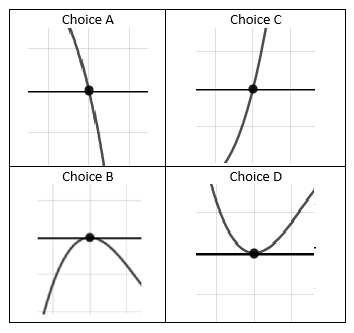
\includegraphics[scale=0.75]{zeroBehaviorOptions.png}
\end{center}

\begin{multipleChoice}
    \choice A Choice A \\
    \choice[correct] B Choice B \\
    \choice C Choice C \\
    \choice D Choice D
\end{multipleChoice}

\end{question}

% Q8
\begin{question}
Choose the option that describes the behavior at $x = \sage{zeroOnDisplay8}$ of the polynomial below.

$$ f(x) = \sage{polynomial8} $$

\begin{center}
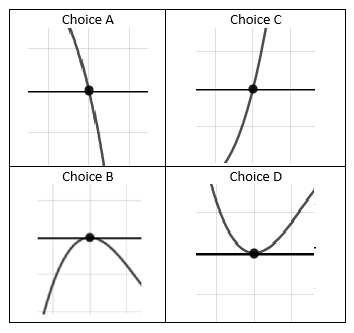
\includegraphics[scale=0.75]{zeroBehaviorOptions.png}
\end{center}

\begin{multipleChoice}
    \choice A Choice A \\
    \choice B Choice B \\
    \choice C Choice C \\
    \choice[correct] D Choice D
\end{multipleChoice}

\end{question}

% Q9
\begin{question}
Choose the option that describes the behavior at $x = \sage{zeroOnDisplay9}$ of the polynomial below.

$$ f(x) = \sage{polynomial9} $$

\begin{center}
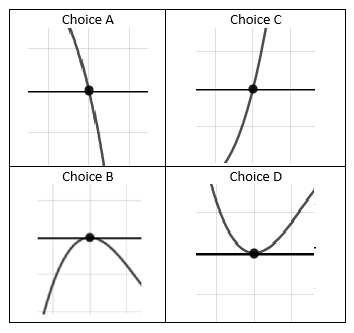
\includegraphics[scale=0.75]{zeroBehaviorOptions.png}
\end{center}

\begin{multipleChoice}
    \choice A Choice A \\
    \choice B Choice B \\
    \choice[correct] C Choice C \\
    \choice D Choice D
\end{multipleChoice}

\end{question}

\end{document}
